\section{Manejo de Guardas: \\ Guard Providers}
\label{sec:guard_providers}
Las guardas son un componente importante de las RdP no autónomas utilizadas para
modelar los sistemas concurrentes (ver
sección~\ref{guardas}). Las mismas
permiten relacionar la RdP con el estado del medio, y representar condiciones de
ejecución síncronas propias del mismo sistema (ver
sección~\ref{sec:arquitectura_alto_nivel}).

El monitor de petri ofrece una interfaz para realizar el seteo del valor
de una guarda. De esta manera se permite al usuario indicar directamente
dicho valor. Sin embargo, el uso de esta alternativa trae aparejada una pérdida
de la inversión de control. Esto se debe a que se puede modificar el estado
de la red de manera directa y en cualquier instante, permitiendo al usuario tomar
parte del control de la ejecución.

Para lidiar con este problema se propone el concepto de Guard Provider. Un Guard
Provider es un método asociado a una guarda que retorna una variable de tipo
boolean. Este método es llamado automáticamente luego de ejecutar un controlador
de acción que requiera modificar dicha guarda. Para lograr la llamada automática
a un Guard Provider se utiliza reflection (ver sección~\ref{reflection}). La
finalidad de un método Guard Provider retornar el valor que debe
tomar la guarda asociada. 

El concepto de Guard Provider permite limitar el acceso a las
guardas. En consecuencia, la modificación de una de ellas se realiza sólo tras
realizar las acciones que deben modificar en la RdP el estado representado por
dicha guarda. El usuario tiene la capacidad de definir la lógica que da el
valor a la guarda, pero el monitor conserva la decisión de ejecución del Guard
Provider, ya que la misma esta asociada a la ejecución de los controladores de acciones (ver
sección~\ref{sec:controladores_de_acciones})

\begin{figure}[H]
	\centering
	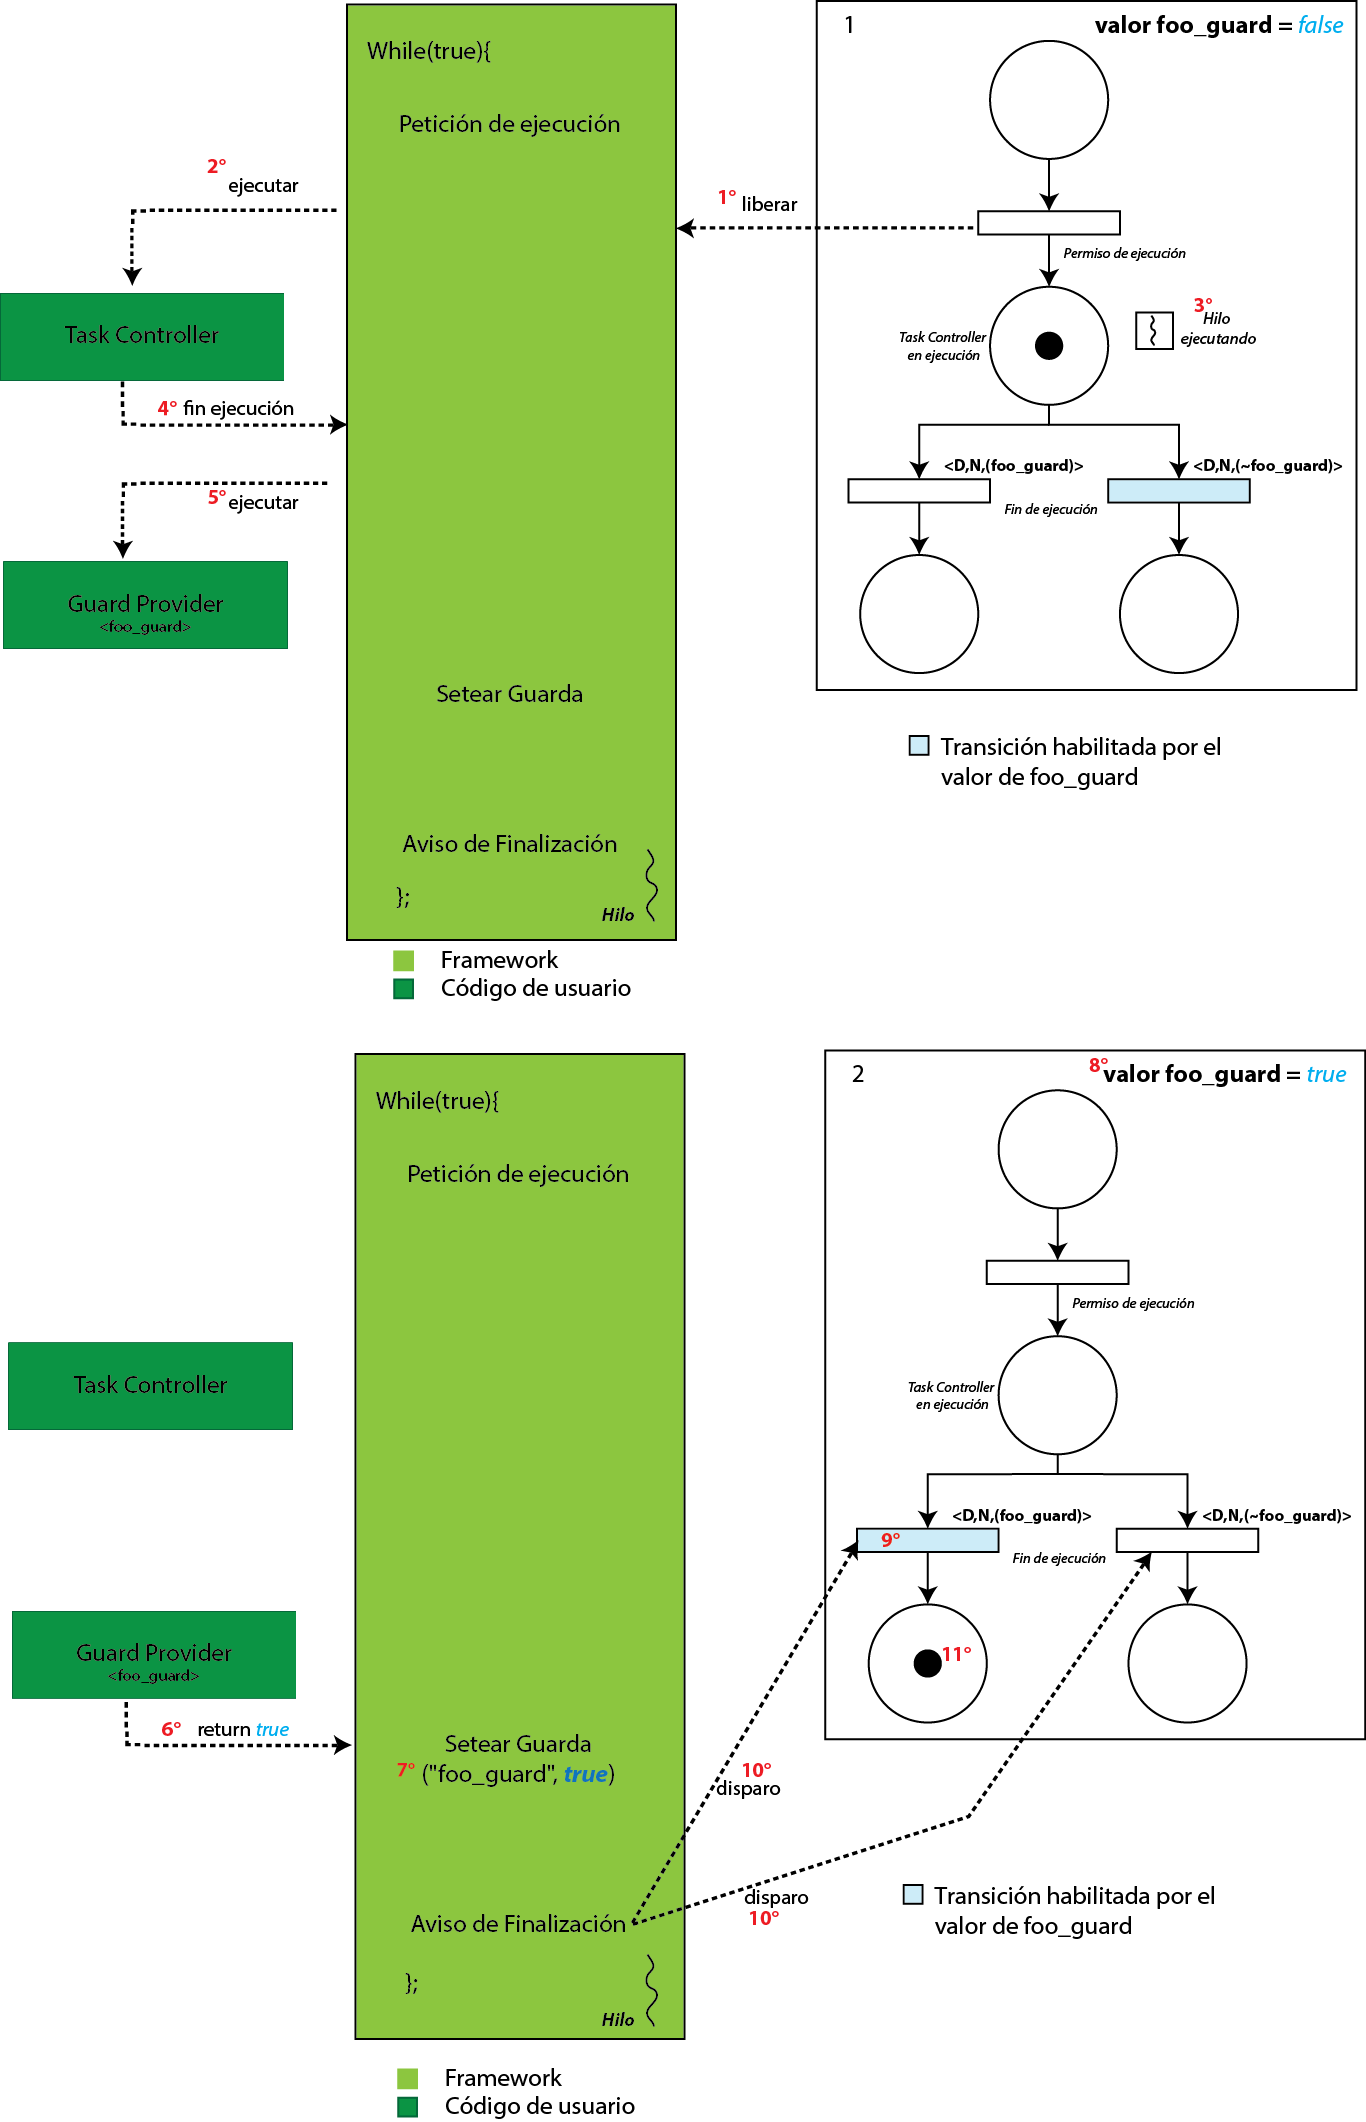
\includegraphics[width=120mm]{ejecucion_guard_provider}
	\caption{Pasos de la Ejecución de un Guard Provider asociado a un Task
	Controller }
	\label{fig:ejecucion_guard_provider}
\end{figure}